\documentclass{standalone}
\usepackage{tikz}
\usetikzlibrary{positioning,shapes.symbols}
%
\begin{document}

\begin{tikzpicture}
  \node[anchor=south west,inner sep=0] (image) at (0,0) {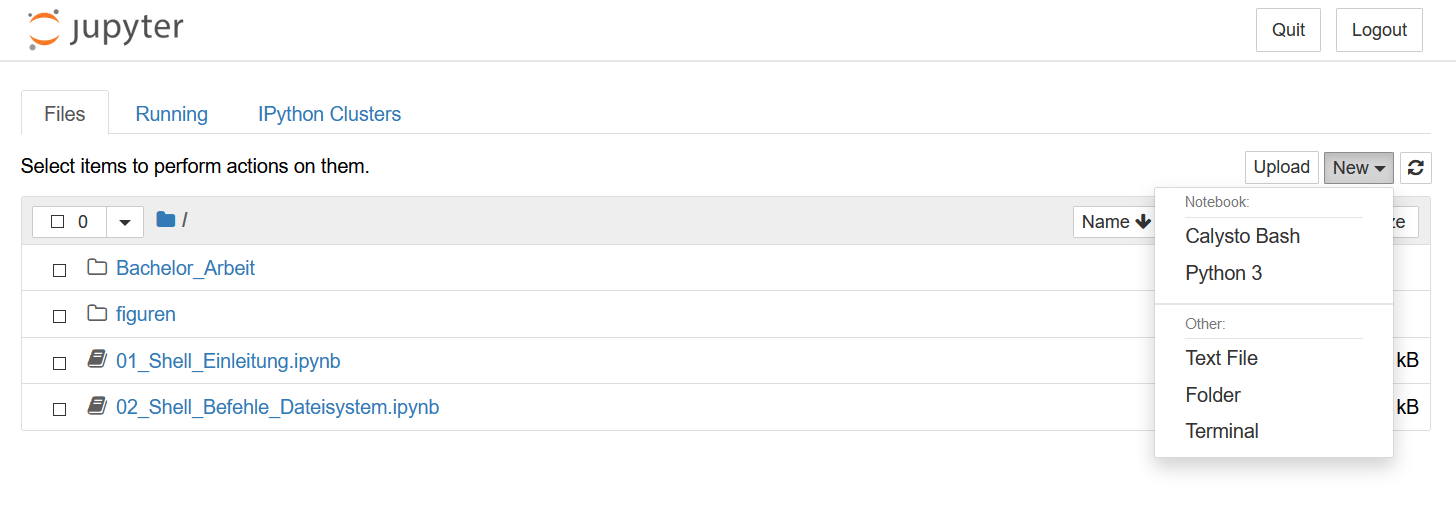
\includegraphics[width=5cm]{figuren/Jupyter_screen.png}};
  %
  \begin{scope}[x={(image.south east)},y={(image.north west)}]
    %\draw[help lines, very thin, step=0.02] (0,0) grid (1,1);
    %\draw[help lines,thin,xstep=.1,ystep=.1] (0,0) grid (1,1);
    %\foreach \x in {0,1,...,9} { \node [anchor=north] at (\x/10,0) {0.\x}; }
    %\foreach \y in {0,1,...,9} { \node [anchor=east] at (0,\y/10) {0.\y}; }
    %\draw[<-] (0.45,0.4) -- (1.1,1.1) node[above] {marmot's crystal ball};
    \node[fill = blue!10, font=\tiny, align = center] (notebook) at (0.3, 1.0) {Lektion \\ starten};
    \node[fill = red!10, font=\tiny, align = center] (terminal) at (0.6, 1.0) {Linux-Terminal \\ starten};
    \draw[red, thick] (0.8, 0.15) rectangle (0.88, 0.23);
    \draw[blue, thick] (0.03, 0.28) rectangle (0.27, 0.35);
    \draw[-latex, blue, thick] (notebook) to (0.15, 0.35);
    \draw[-latex, red, thick] (terminal) to (0.84, 0.23);
  \end{scope}
\end{tikzpicture}

\end{document}
